\section{Auswertung}
\label{sec:Auswertung}
%\rot{
%  Sweep und Horizontal sind vertauscht gewesen. \\
%  Horizontal max 1A, → 1 Drehung 0,1A \\
%  Sweep max 3A → 1 Drehung 0,3A
%}

\subsection{Erdmagnetfeld}
Die Kompensation des Erdmagnetfeldes mit der Vertikalspule führt zu
einem Spulenstrom von $\SI{0.215}{\ampere}$.
Daraus ergibt sich mit den Daten in Tabelle \ref{tab:spulen}
und Gleichung \eqref{eqn:helmholtz}
\begin{equation}
  B_\text{V} = \left(\frac{4}{5}\right)^{\!\!\frac{3}{2}}
    \frac{μ_0 \cdot 20 \cdot \SI{0.215}{\ampere}}{\SI{11.735}{\centi\meter}}
  = \input{build/messung-b.tex}
\end{equation}
für die Vertikalkomponente des Erdmagnetfeldes.
Der Literaturwert \cite{erdmagnetfeld} beträgt
\begin{equation}
  B_\text{lit} = \SI{45.136}{\micro\tesla}\,.
\end{equation}

\subsection{Kernspins über die Resonanzen}
\label{sec:5.2}
Die Messwerte sind in Tabelle \ref{tab:messung-c} aufgetragen.
Von diesen ausgehend wird mit der Skalierung des Potentiometers von 0,3 multipliziert.
Die errechneten Stromstärken werden dann mit der Gleichung \eqref{eqn:helmholtz}
in die entsprechenden B-Feldstärken umgerechnet.
In der Abbildung \ref{fig:messung-c} sind diese gegen die Frequenz der Sinuswelle aufgetragen.

Die Bezeichung erfolgt anhand von Abbildung \ref{fig:messung-c-oszi} von links nach rechts.

Mit der Ausgleichsgeraden
\begin{equation}
  B_i = m_i \cdot f + b_i
\end{equation}
liefert \texttt{scipy} die Werte
\begin{align}
  \input{build/messung-c-m1.tex} \\
  \input{build/messung-c-b1.tex} \\
  \input{build/messung-c-m2.tex} \\
  \input{build/messung-c-b2.tex} \\
  \input{build/messung-c-m3.tex} \\
  \input{build/messung-c-b3.tex}\,.
\end{align}
Nach Gleichung \eqref{eqn:B_M_Theorie} sind die $m_i$
die Proportionalitätsfaktoren zwischen $f$ und $B$.
Mit umstellen zu
\begin{equation}
  g_{(f,i)} = \frac{4 \mpi \cdot \symup{m}_{\me}}{\me \cdot m_i}
\end{equation}
folgen die Werte
\begin{align}
  \input{build/messung-c-gf2.tex} \\
  \input{build/messung-c-gf3.tex}\,.
\end{align}
Mit der Gleichung
\begin{equation}
  I = \frac{g_j}{(4 \cdot g_3} - 1 +
    \sqrt{\left(\frac{g_j}{4 \cdot g_f} -1\right)^{\!\!2} + \frac{3}{4}
      \cdot \left(\frac{g_j}{g_f} -1\right)}
\end{equation}
ergeben sich die Kernspins zu
\begin{align}
  \input{build/messung-c-i2.tex} \\
  \input{build/messung-c-i3.tex}\,.
\end{align}
Durch einen Vergleich mit der Literatur \cite{opticalpumping} kann
das Minimum 2 $^{87}\text{Rb}$ mit einem Kernspin von $\sfrac{3}{2}$
und das Minimum 3 $^{85}\text{Rb}$ mit einem Kernspin von $\sfrac{5}{2}$
zugeordnet werden.

\begin{figure}
  \centering
  \includegraphics[width=0.8\textwidth]{build/messung-c.pdf}
  \caption{Darstellung der Daten aus Messung c).}
  \label{fig:messung-c}
\end{figure}

\begin{figure}
  \centering
  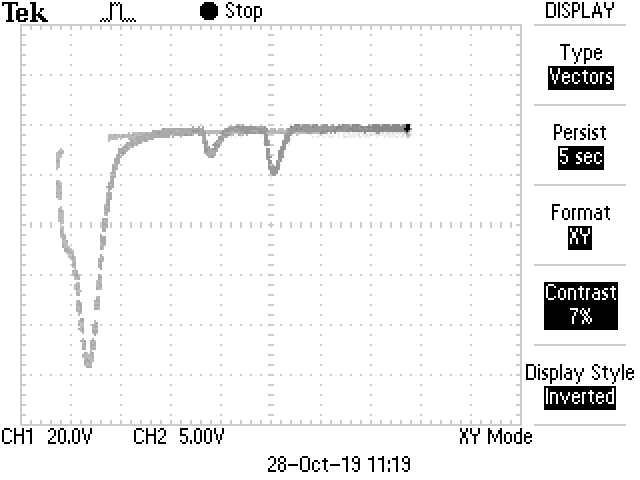
\includegraphics[width=0.8\textwidth]{data/messung-f/f1.JPG}
  \caption{Oszilloskopbild der Messung. (Messauftrag f)\newline
  Von links nach rechts: Min. 1 → Min. 2 → Min. 3}
  \label{fig:messung-c-oszi}
\end{figure}

\begin{table}
  \centering
  \caption{Messwerte und Magnetfeldstärken in der Messung c).}
  \label{tab:messung-c}
  \sisetup{table-format=1.2}
  \begin{tabular}{S[table-format=4.0] S[table-format=1.3] S S S[table-format=2.2] S S[table-format=2.2]}
    \toprule
    & \multicolumn{2}{c}{Minimum 1} & \multicolumn{2}{c}{Minimum 2}& \multicolumn{2}{c}{Minimum 3} \\
    {$f\:/\:\si{\kilo\hertz}$}
    & {$I_1\:/\:\si{\ampere}$} & {$B_1\:/\:\si{\micro\tesla}$}
    & {$I_2\:/\:\si{\ampere}$} & {$B_2\:/\:\si{\micro\tesla}$}
    & {$I_3\:/\:\si{\ampere}$} & {$B_3\:/\:\si{\micro\tesla}$} \\
    \midrule
     100 & 0.024 & 21.05 & 0.040 &  35.08 & 0.049 &  42.97 \\
     200 & 0.024 & 21.05 & 0.057 &  49.99 & 0.074 &  64.90 \\
     300 & 0.024 & 21.05 & 0.074 &  64.90 & 0.099 &  86.82 \\
     400 & 0.024 & 21.05 & 0.094 &  82.43 & 0.125 & 109.62 \\
     500 & 0.024 & 21.05 & 0.108 &  94.71 & 0.150 & 131.55 \\
     600 & 0.024 & 21.05 & 0.125 & 109.62 & 0.175 & 153.47 \\
     700 & 0.024 & 21.05 & 0.142 & 124.53 & 0.200 & 175.39 \\
     800 & 0.024 & 21.05 & 0.158 & 138.56 & 0.226 & 198.19 \\
     900 & 0.024 & 21.05 & 0.175 & 153.47 & 0.251 & 220.12 \\
    1000 & 0.024 & 21.05 & 0.193 & 169.25 & 0.276 & 242.04 \\
    \bottomrule
  \end{tabular}
\end{table}
\FloatBarrier
\subsection{Isotopenverhältnis}
Das Verhältnis wird über die Stärke der Pulse ermittelt,
dieses beträgt
\begin{equation}
  \frac{7}{11} = 0,\overline{63}\,,\quad\text{bzw.}\quad\frac{11}{7} = 1,57
\end{equation}
Es ergibt sich für die relativen Anteile
\begin{align}
  ^{87}\text{Rb}\!:\quad&\SI{39}{\percent} \\
  ^{85}\text{Rb}\!:\quad&\SI{61}{\percent}\,.
\end{align}
Die Literaturwerte \cite{opticalpumping} sind
\begin{align}
  ^{87}\text{Rb}\!:\quad&\SI{28}{\percent} \\
  ^{85}\text{Rb}\!:\quad&\SI{72}{\percent}\,.
\end{align}

\subsection{Quadratischer Zeeman-Effekt}
Nach Gleichung \eqref{eqn:zeequadr} kann der quadratische Zeeman-Effekt zu
\begin{align}
  \laplace E_{85} &= \SI{2.01e-24}{\joule} &\input{build/messung-h-dE3.tex} \\
  \laplace E_{87} &= \SI{4.53e-24}{\joule} &\input{build/messung-h-dE2.tex}
\end{align}
bestimmt werden.

\subsection{Schwing-Kernspin}
Die Funktion
\begin{equation}
  T = a + \frac{b}{x - c}
\end{equation}
wird, wieder mit \texttt{scipy} an die genommenen Messwerte gefittet.
Dabei ist $x$ die RF-Amplitude.
Die Parameter sind für die blaue Kurve
\begin{align}
  \input{build/messung-i-a1.tex} \\
  \input{build/messung-i-b1.tex} \\
  \input{build/messung-i-c1.tex}
  \intertext{und für die grüne Kurve}
  \input{build/messung-i-a2.tex} \\
  \input{build/messung-i-b2.tex} \\
  \input{build/messung-i-c2.tex}\,.
\end{align}
Das Verhältnis der Parameter $b_i$ beträgt
\begin{align}
  \frac{b_2}{b_1} &= \input{build/messung-i-bb.tex}\,,
  \intertext{der Literaturwert \cite{anleitung} ist}
  \frac{b_2}{b_1} &= 1,5\,.
\end{align}
\begin{figure}[ht]
  \centering
  \includegraphics[width=0.8\textwidth]{build/messung-i.pdf}
  \caption{Messwerte der Abschwingvorgänge.}
  \label{fig:messung-i.pdf}
\end{figure}

\FloatBarrier
